\section{Experiments and Analysis}
\label{sec:exp}

After presenting the method design, this section validates the effectiveness of the proposed framework through simulation. The experiments are organized along several interconnected levels. First, the JPS-based improved A* planner is compared with common baselines in terms of global path-finding efficiency and path quality. Second, the sensitivity of MMAS-VND-CL to key hyperparameters is examined. Third, ablation experiments isolate the contribution of each constituent mechanism. Finally, different traveling-salesman solvers are combined with the improved A* planner to compare complete multi-goal traversal performance. All comparisons are repeated independently multiple times under a unified parameter policy, so that solution quality and statistical stability are both accounted for.

\begin{figure*}[!htbp]
\centering
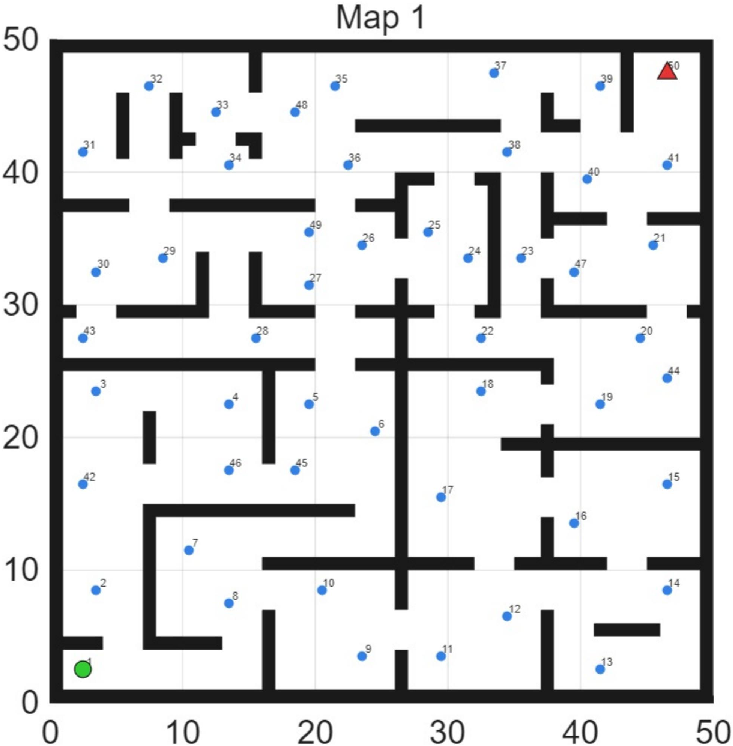
\includegraphics[height=3.7cm]{figures/Map_1}\hfil
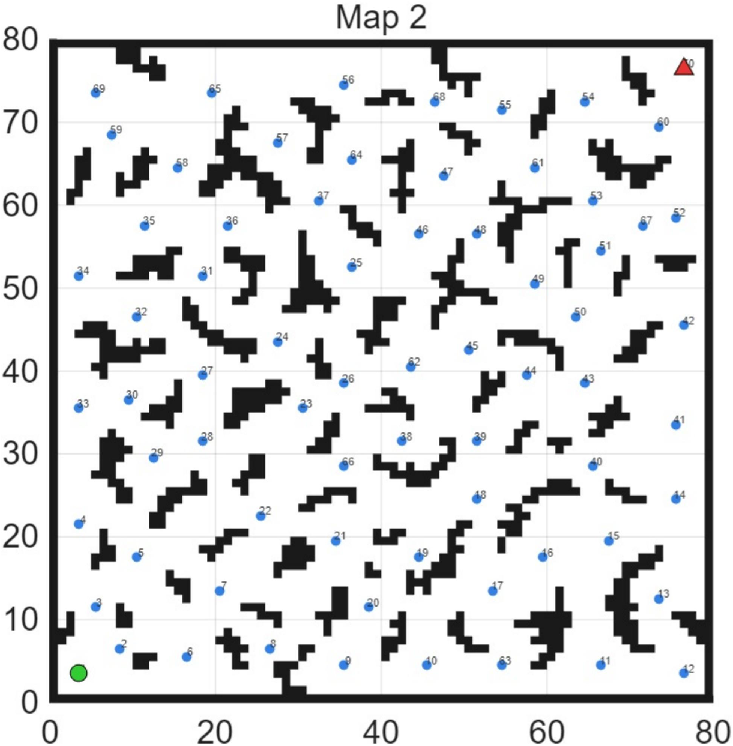
\includegraphics[height=3.7cm]{figures/Map_2}\hfil
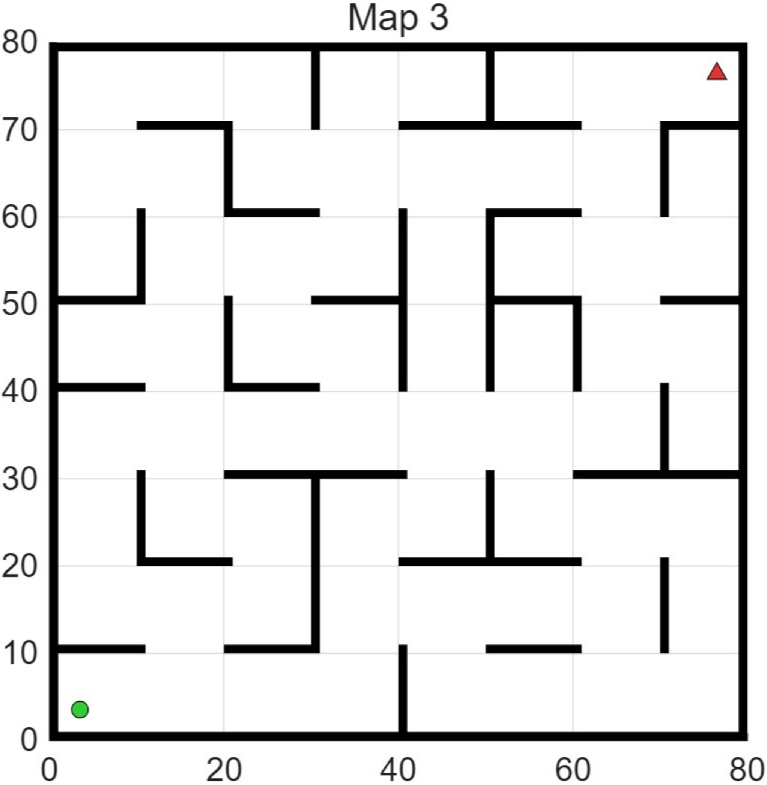
\includegraphics[height=3.7cm]{figures/Map_3}\hfil
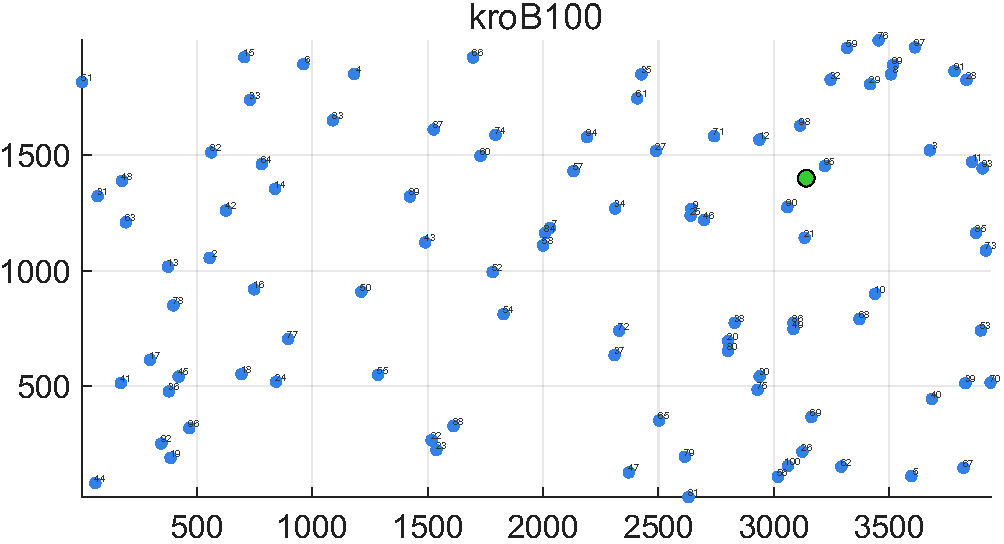
\includegraphics[height=3.7cm]{figures/Map_kroB100}
\caption{Schematic of the experimental environments. In Map~1 and Map~2, green circles denote the start point, red triangles the goal point, and blue numbered points the intermediate targets for multi-goal traversal; Map~3 provides only the start and goal; kroB100 shows the planar distribution of 100 cities, with green circles marking the endpoints of the open path.}
\label{fig:env_maps}
\end{figure*}

\subsection{Experimental Setup}

All experiments were conducted on a computer equipped with an Intel Core Ultra 5 125H processor and 32~GB of memory, using MATLAB R2025b as the software environment.

To cover different obstacle morphologies and problem scales, two classes of experimental scenarios were constructed, as illustrated in Fig.~\textcolor{blue}{\ref{fig:env_maps}}. One class consists of obstacle-laden grid maps (Map~1, Map~2, and Map~3), used to examine obstacle-avoiding path finding and multi-goal traversal. The other class is the standard TSPLIB instance kroB100, used solely to examine large-scale combinatorial ordering capability. In the figure, green circles denote the start point, red triangles the goal point, and blue numbered points the intermediate targets in the multi-goal traversal experiments. Map~1 and Map~2 simultaneously provide the intermediate targets required for multi-goal traversal; in the global path-planning comparison of Section~\textcolor{blue}{\ref{subsec:exp_plan}}, only the start and goal of each map are used for point-to-point planning, and no visit-order optimization over intermediate targets is involved.

The specific environment characteristics are as follows.

\begin{enumerate}

\item Map~1: a $50\times 50$ grid environment. Obstacles are dominated by relatively long horizontal and vertical wall segments arranged in a staggered manner, forming several corridor-connected ``room''-like cavities. The layout is broadly reminiscent of an urban block or an indoor partitioned floor plan. Free-space connectivity is acceptable, but straight passages are repeatedly interrupted by walls, which is suitable for examining detour behavior and search efficiency under moderate obstacle density.

\item Map~2: an $80\times 80$ grid environment. Obstacles appear as irregular, high-density fragmented patches, and the free space is cut into numerous narrow, winding passages whose local traversability depends heavily on short-range obstacle avoidance. Compared with Map~1, the search exhibits more branching and a more pronounced staircase effect along the path, making the map useful for assessing robustness in cluttered environments. It likewise contains the start point, the goal point, and numbered intermediate targets.

\item Map~3: an $80\times 80$ maze environment. Wall segments are longer and largely orthogonal, constituting typical maze-like corridors with narrow, elongated passages and frequent turns. No intermediate targets are placed; the map is used only for the global path-planning comparison, so as to highlight performance differences among path-finding algorithms in a structured maze.

\item kroB100: the standard 100-city TSPLIB instance. Cities are given by planar coordinates without grid obstacles, and the focus is on the visit-order optimization of a large set of targets. In this paper, both the start and the goal are set to city~1, so that the open path degenerates into a tour and can be compared directly with the published TSPLIB optimal tour length of 22141, serving as a calibration benchmark for combinatorial search capability at a scale of about one hundred points. Open-traversal settings with distinct start and goal are covered by the multi-goal traversal experiments on Map~1 and Map~2.

\end{enumerate}

The scales of the multi-goal traversal instances are as follows. Map~1 uses 50 navigation points including the start and the goal, and Map~2 uses 70 navigation points including the start and the goal. The start and the goal are respectively the first and last points of each instance's navigation-point sequence, and the grid coordinates of the navigation points are given by the numbered annotations in Fig.~\textcolor{blue}{\ref{fig:env_maps}}. The kroB100 instance contains all 100 cities. The safety-distance threshold used for path simplification is $d_{\mathrm{safe}} = 0.4$ (grid units), and the spline-smoothing density takes the default value $\rho = 10$.

\begin{table}[!ht]
\caption{Default Parameter Settings of the Proposed Algorithm}
\label{tab:params}
\centering
\scriptsize
\begin{tabular}{lccc}
\toprule
Module & Parameter & Symbol & Value \\
\midrule
\multirow{6}{*}{Original params}
& Number of ants & $n_{\mathrm{ants}}$ & 40 \\
& Pheromone weight & $\alpha$ & 1 \\
& Heuristic weight & $\beta$ & 2.0 \\
& Evaporation rate & $\rho$ & 0.25 \\
& Deposit constant & $Q$ & 225 \\
& Initial pheromone & $\tau_0$ & 0.1 \\
\midrule
\multirow{1}{*}{ACS}
& Greedy probability & $q_0$ & 0.45 \\
\midrule
\multirow{6}{*}{VND}
& Local search ratio & $y_{\max}$ & 0.4 \\
& \makecell{Local search transition\\interval} & $[x_L, x_R]$ & $[0, 30]$ \\
& Elite ratio & $r_{\mathrm{elite}}$ & 0.7 \\
& Candidate list size & $k$ & 9 \\
& Local search ratio lower bound & $y_{\min}$ & 0.0 \\
& S-curve steepness & $a$ & 2.0 \\
\midrule
\multirow{4}{*}{Adaptive stopping}
& Homogeneity threshold & $\varepsilon_{\mathrm{CV}}$ & $10^{-3}$ \\
& Stagnation limit & $\mathrm{stagn}_{\max}$ & 70 \\
& Minimum iterations & $\mathrm{minIter}$ & 30 \\
& Maximum iterations & $n_{\mathrm{iter}}$ & 800 \\
\bottomrule
\end{tabular}
\end{table}

Regarding the number of repetitions and the statistical protocol: in the global path-planning comparison, each algorithm is run 10 times on each map and the average computation time is reported. In the traveling-salesman-related experiments, each configuration is run 40 times, and the best cost, the mean convergence cost with standard deviation, the computation time, and the success rate are reported. The computation time of the traveling-salesman-related experiments is the solver time on a precomputed cost matrix and does not include the $O(N^2)$ cost-matrix construction or path post-processing.

\begin{figure*}[!htbp]
\centering
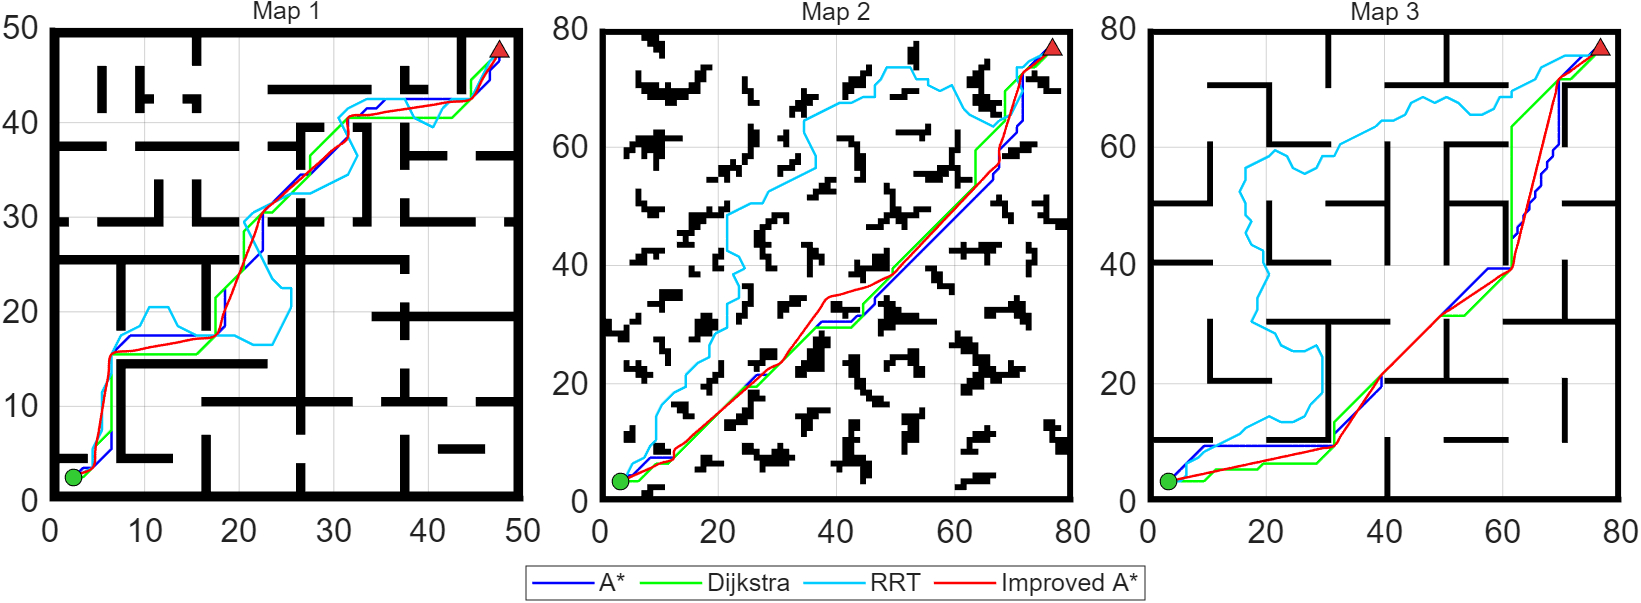
\includegraphics[width=0.92\textwidth]{figures/DifPathPlan_pathCompare}
\caption{Path-planning results of the four algorithms on the three maps.}
\label{fig:plan_paths}
\end{figure*}

For the parameter settings, the main parameters of the proposed MMAS-VND-CL algorithm take the default values listed in Table~\textcolor{blue}{\ref{tab:params}} throughout the paper.

The evaluation metrics include path length, computation time, number of expanded nodes (global planning only), best cost, mean convergence cost, success rate, and standard deviation. The sources of the reference best costs fall into two categories. The reference value of 22141 for kroB100 is the optimal tour length published by TSPLIB and is therefore an externally certified value. The reference values for Map~1 and Map~2 are 352.56 and 623.78, respectively, and correspond to the best observed values over all algorithms and all runs in this experiment. The success rate is defined as the fraction of runs that attain the reference best cost. Because the reference values for Map~1 and Map~2 come from observation rather than certified optima, a baseline success rate of 0\% should be understood as not attaining the best known value of this experiment, rather than as the absence of a feasible solution.

\subsection{Global Path Planning Comparison}
\label{subsec:exp_plan}

This group of experiments compares the proposed JPS-based improved A* planner with three baselines, namely conventional A*, Dijkstra, and RRT, in terms of path length, computation time, and number of expanded nodes, so as to assess path-finding quality and search efficiency. Each planner is run independently 10 times on Map~1, Map~2, and Map~3, and the average computation time is taken. The results are summarized in Table~\textcolor{blue}{\ref{tab:plan}}. Path visualizations and the length and time comparisons are shown in Fig.~\textcolor{blue}{\ref{fig:plan_paths}}--\textcolor{blue}{\ref{fig:plan_time}}, respectively. Overall, the proposed method simultaneously achieves the shortest paths, fewer node expansions, and shorter computation times on all three maps. Sampling-based methods may trade path quality for extremely short computation time in individual scenarios, while fragmented obstacles weaken the pruning advantage of JPS relative to conventional A*. The following discussion elaborates on these points by combining the metrics, the conditions, and the algorithmic mechanisms.

\begin{table}[!ht]
\caption{Global Path-Planning Performance Comparison}
\label{tab:plan}
\centering
\footnotesize
\setlength{\tabcolsep}{4pt}
\begin{tabular}{ccccc}
\toprule
Algorithm & Map & Path Length & Time (ms) & Expanded Nodes \\
\midrule
\multirow{3}{*}{Improved A*}
& Map 1 & 72.93 & 2.45 & 70 \\
& Map 2 & 108.17 & 11.85 & 415 \\
& Map 3 & 113.33 & 4.31 & 48 \\
\midrule
\multirow{3}{*}{A*}
& Map 1 & 76.53 & 6.14 & 811 \\
& Map 2 & 111.44 & 29.19 & 1979 \\
& Map 3 & 119.64 & 17.88 & 2796 \\
\midrule
\multirow{3}{*}{Dijkstra}
& Map 1 & 76.53 & 24.26 & 1997 \\
& Map 2 & 111.44 & 202.29 & 5217 \\
& Map 3 & 119.64 & 204.46 & 5664 \\
\midrule
\multirow{3}{*}{RRT}
& Map 1 & 100.80 & 7.42 & --- \\
& Map 2 & 135.40 & 19.33 & --- \\
& Map 3 & 144.07 & 3.69 & --- \\
\bottomrule
\end{tabular}
\end{table}

\begin{figure}[!ht]
\centering
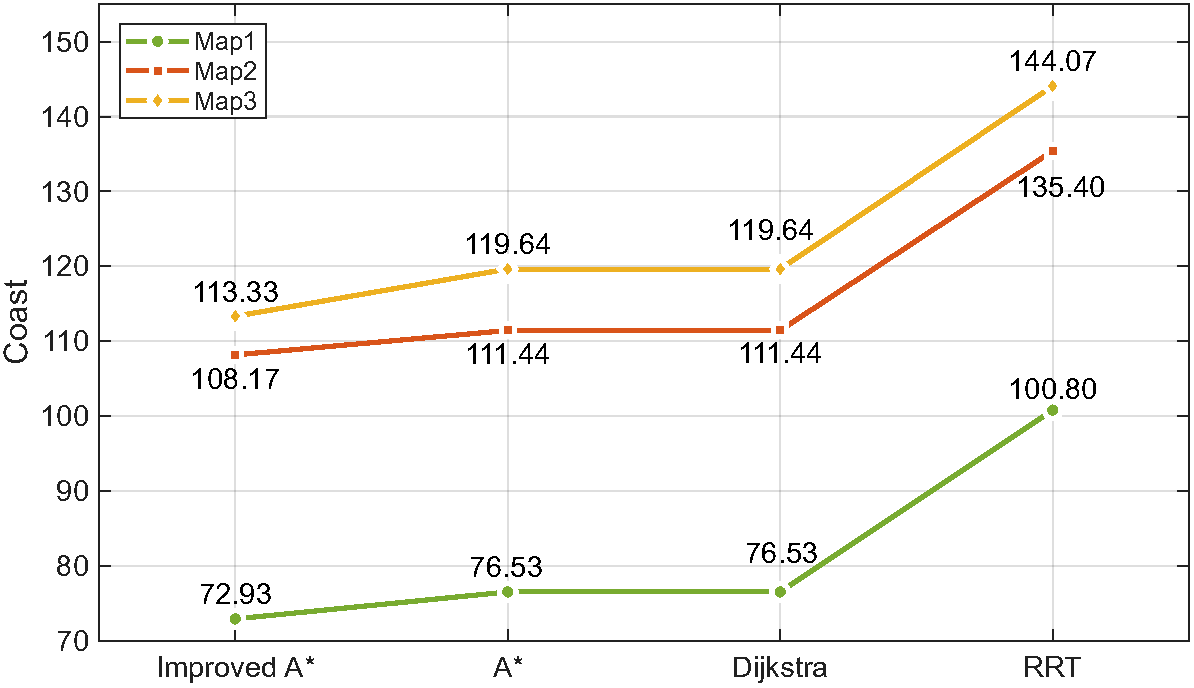
\includegraphics[width=2.5in]{figures/DifPathPlan_CostCompare}
\caption{Path-length comparison of the four algorithms on Map~1, 2, and 3.}
\label{fig:plan_len}
\end{figure}
\begin{figure}[!ht]
\centering
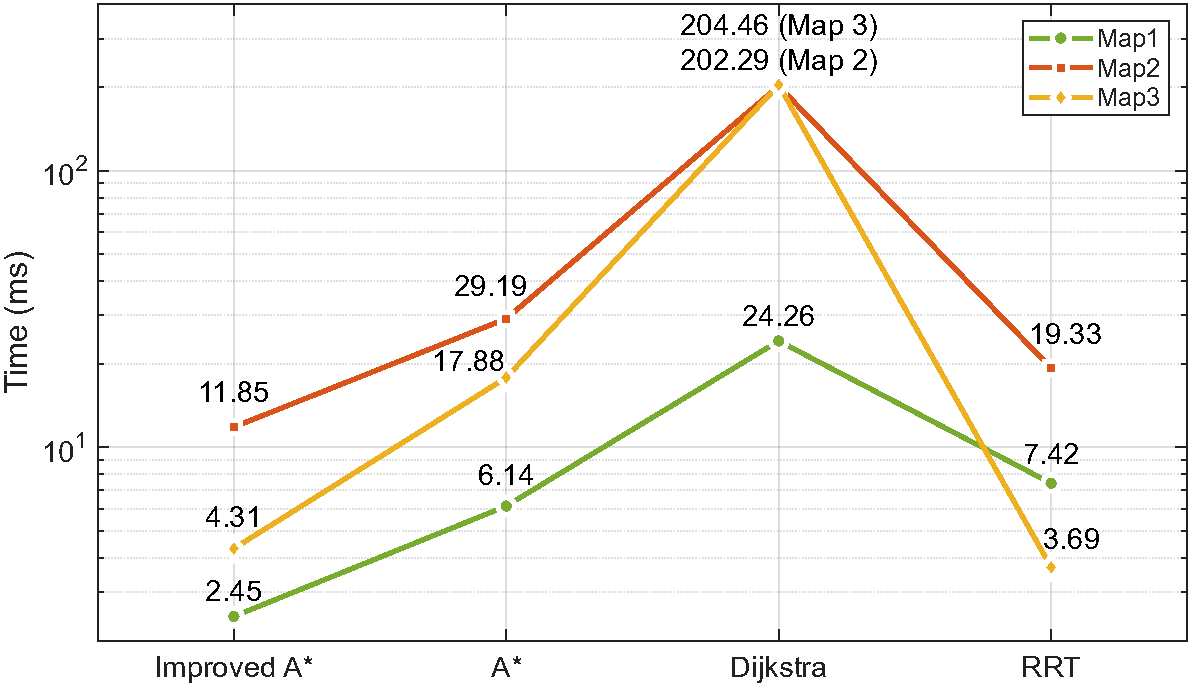
\includegraphics[width=2.5in]{figures/DifPathPlan_TimeCompare}
\caption{Computation-time comparison of the four algorithms on Map~1, 2, and 3.}
\label{fig:plan_time}
\end{figure}

We first consider path length. Table~\textcolor{blue}{\ref{tab:plan}} shows that the proposed method achieves 72.93, 108.17, and 113.33 on Map~1--Map~3, respectively, which are approximately 4.7\%, 2.9\%, and 5.3\% shorter than those of conventional A* and Dijkstra. The line trends in Fig.~\textcolor{blue}{\ref{fig:plan_len}} are consistent with the table, indicating that the advantage is not an isolated coincidence. It should be noted that, under an admissible heuristic, conventional A* and Dijkstra produce the optimal polyline in the grid metric; the fact that their lengths coincide confirms that both have reached the discrete optimum. The shorter length of the proposed method is mainly not because ``another shorter grid path was found,'' but because post-processing turns the staircase-like polyline into a more compact continuous trajectory: safety-aware simplification merges redundant waypoints and trims detours around corners, and spline smoothing further removes jaggedness, bringing the result closer to the physically continuous shortest travel. In other words, the length advantage corresponds directly to the simplification--smoothing mechanism of Section~\textcolor{blue}{\ref{subsec:post}}.

Next, we examine search efficiency. In terms of the number of expanded nodes, the proposed method is far below the two graph-search baselines on all three maps: relative to A*, the reductions are approximately 91.4\%, 79.0\%, and 98.3\%, respectively, and relative to Dijkstra the reduction exceeds about 92\% in every case. This phenomenon can be explained by the symmetry pruning of JPS: jump points are generated only at forced neighbors and at changes of direction, intermediate same-direction cells are no longer inserted into the open set one by one, and the search tree is therefore greatly compressed. On the same map, Dijkstra expands uniformly in all directions, and conventional A*, although guided by a heuristic, still relaxes cell by cell; hence the expanded-node counts differ by an order of magnitude. At the same time, it should be noted objectively that the reduction relative to A* on Map~2 is noticeably smaller than on Map~1 and Map~3: fragmented obstacles make forced neighbors more frequent, the number of jump points rises, and the pruning benefit is partially offset. Even so, an order-of-magnitude advantage over cell-by-cell expansion is maintained overall.

We further compare with sampling-based methods. RRT becomes the fastest method on Map~3 with 3.69~ms. This result must be reported honestly: when the maze corridors are regular and the start and goal are almost connected by a straight line, a random tree may find a feasible solution quickly. The price, however, is a marked degradation in path quality---the RRT path is the longest on all three maps, about 25\%--38\% longer than that of the proposed method. Moreover, as a randomized sampling method, its results fluctuate across runs, which is consistent with the typical weak sampling consistency of such methods. Therefore, under an evaluation protocol that requires both short paths and stable reproducibility, RRT does not constitute a substantive threat to the proposed method. If the task only requires a feasible solution quickly, sampling methods still have their applicable scope.

In summary, the three metrics corroborate one another. The length advantage comes from the approximation of continuous travel by simplification--smoothing, whereas the expansion and time advantages come from the pruning of the search tree by JPS. The two correspond to different mechanisms in the post-processing pipeline and the graph-search kernel, respectively. The relatively narrower pruning gain on Map~2 indicates that forced neighbors in highly cluttered grids weaken the symmetry benefit of JPS, yet both the expanded-node count and the computation time remain comprehensively better than those of cell-by-cell graph search. Future work may consider adaptively adjusting pruning or jump-point generation strategies on highly cluttered maps to further reduce the search overhead in such scenarios.

\subsection{Parameter Sensitivity Analysis}
\label{subsec:exp_sens}

\begin{figure*}[!ht]
\centering
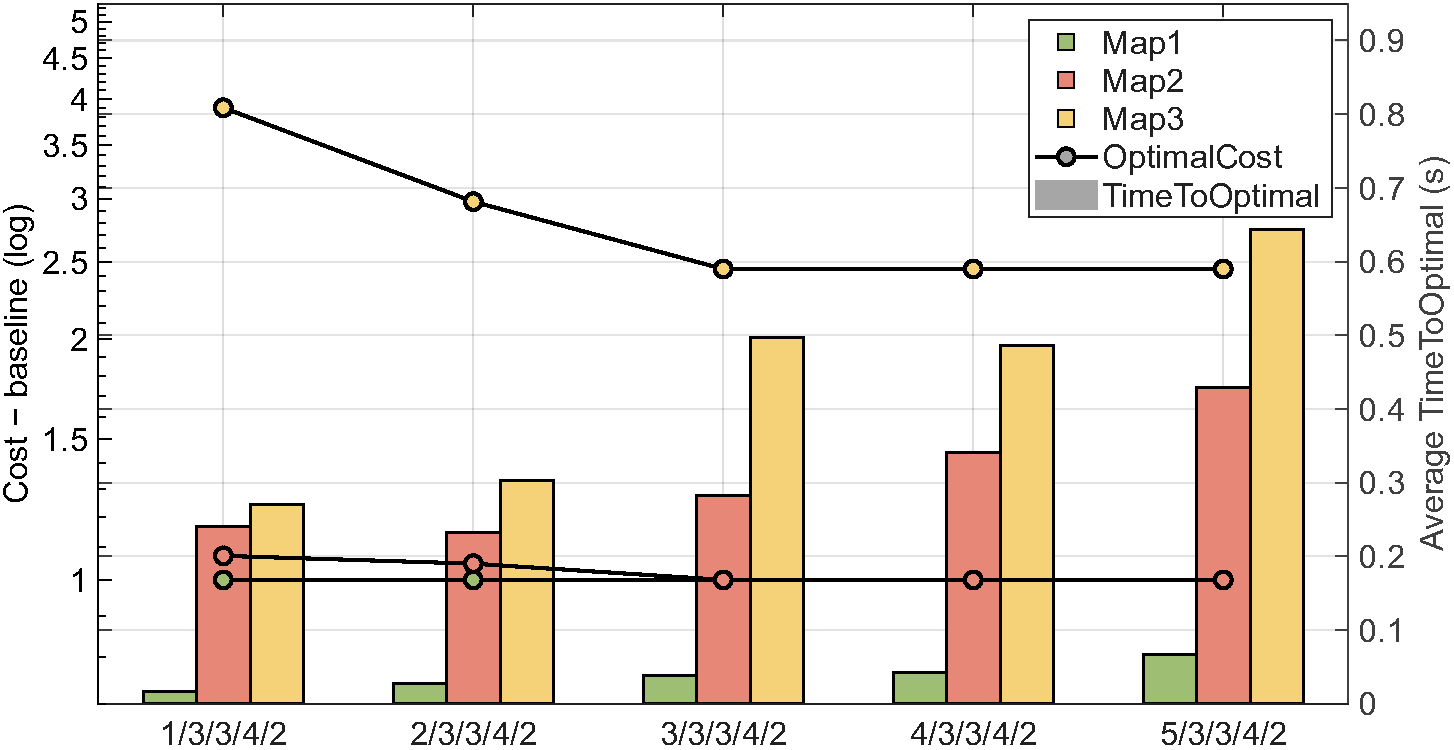
\includegraphics[width=0.32\textwidth]{figures/Sensitivity_Cost&Time_nAnts}\hfil
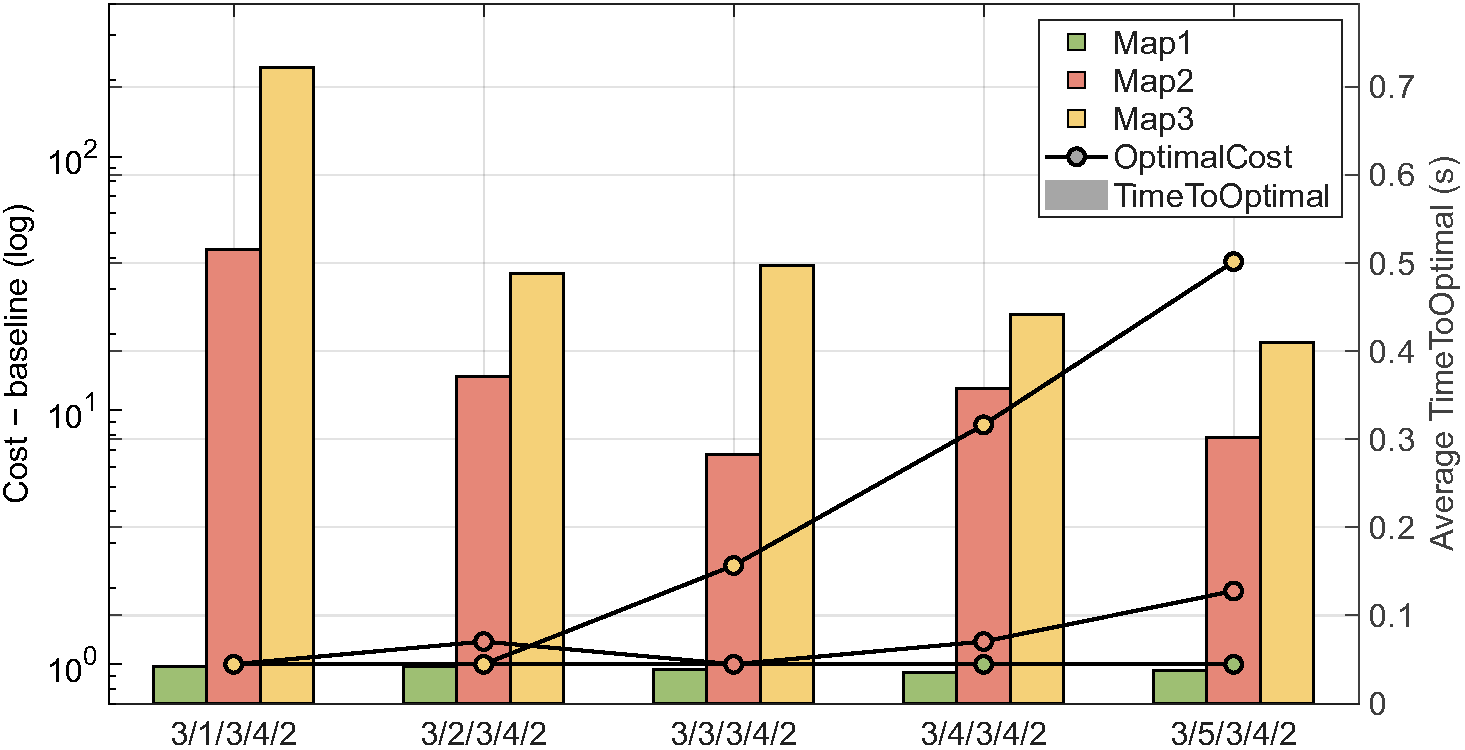
\includegraphics[width=0.32\textwidth]{figures/Sensitivity_Cost&Time_q0}\hfil
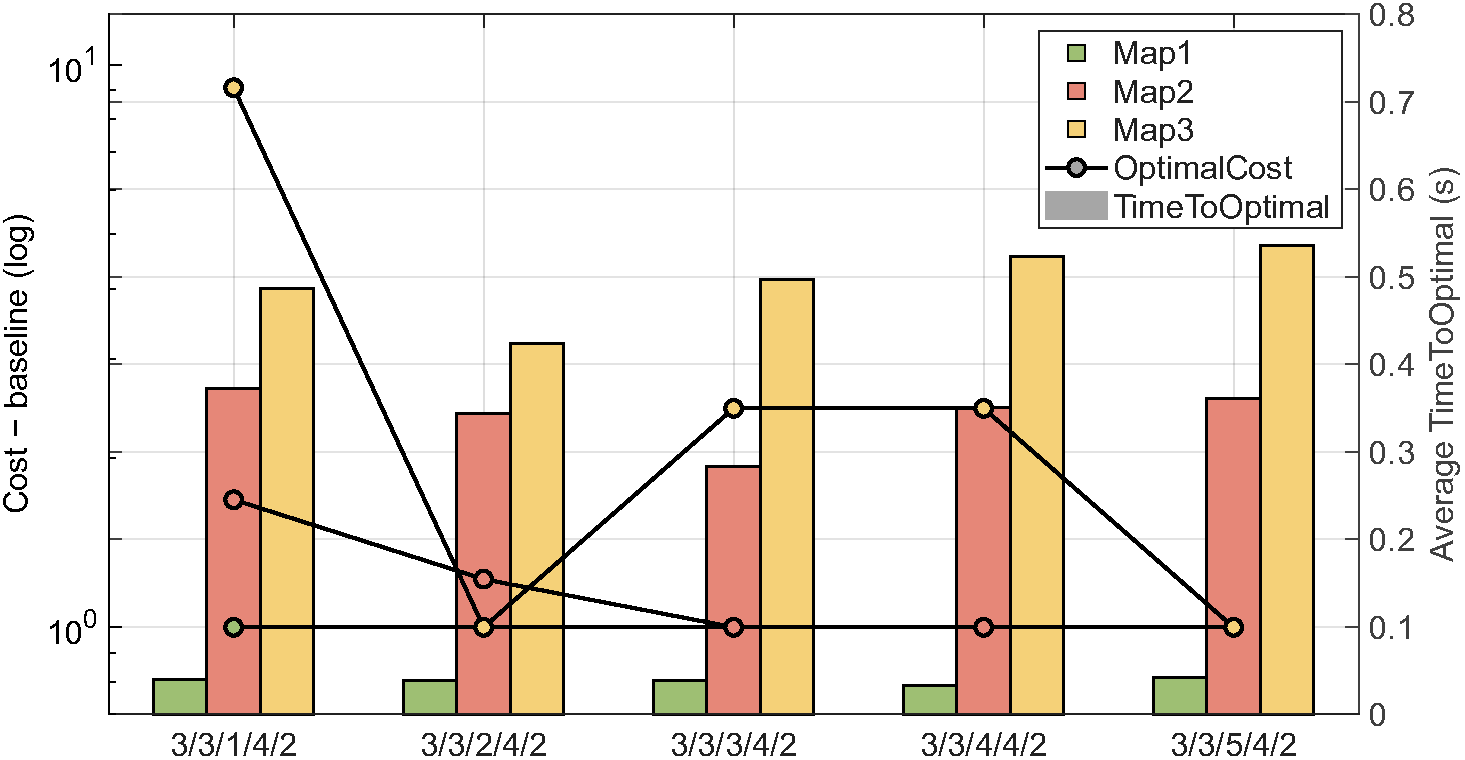
\includegraphics[width=0.32\textwidth]{figures/Sensitivity_Cost&Time_ymax}\\
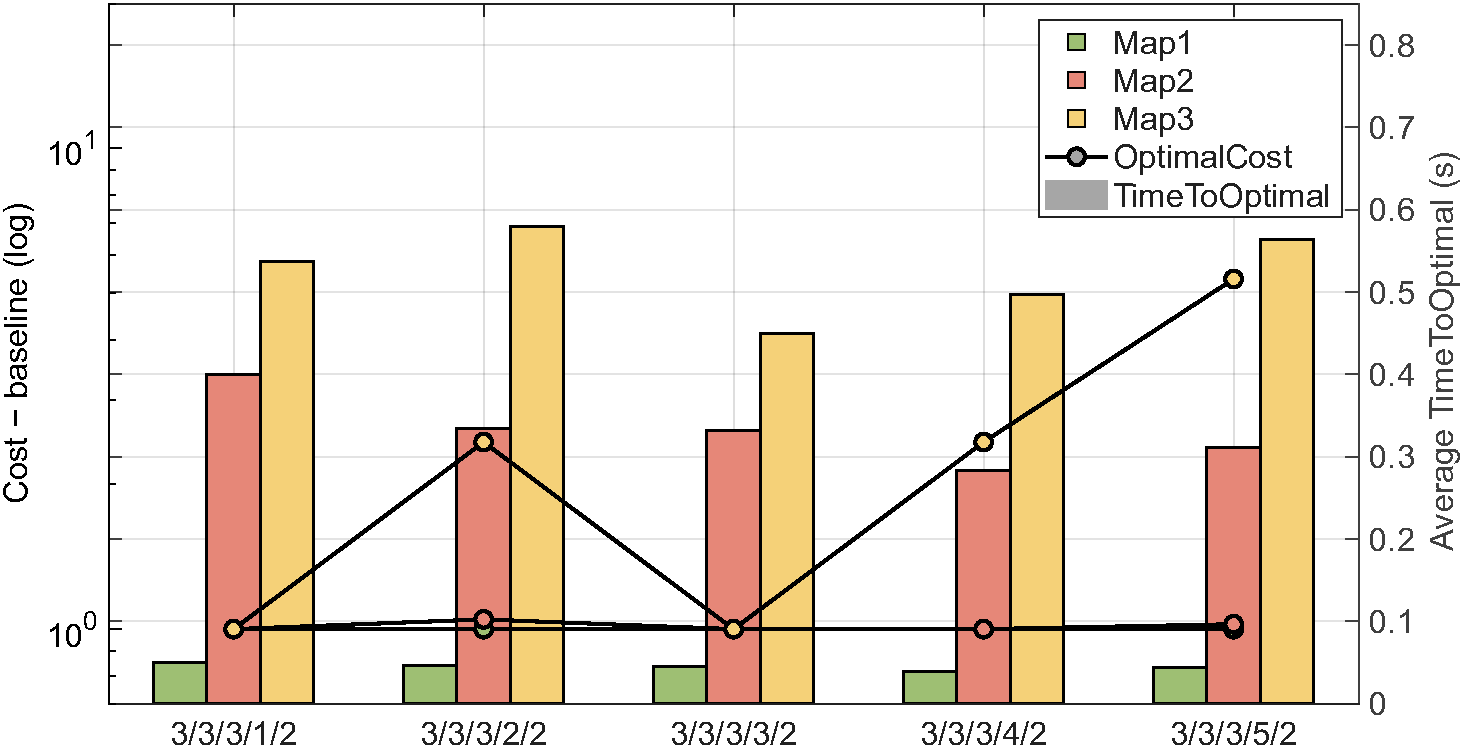
\includegraphics[width=0.32\textwidth]{figures/Sensitivity_Cost&Time_relite}\hfil
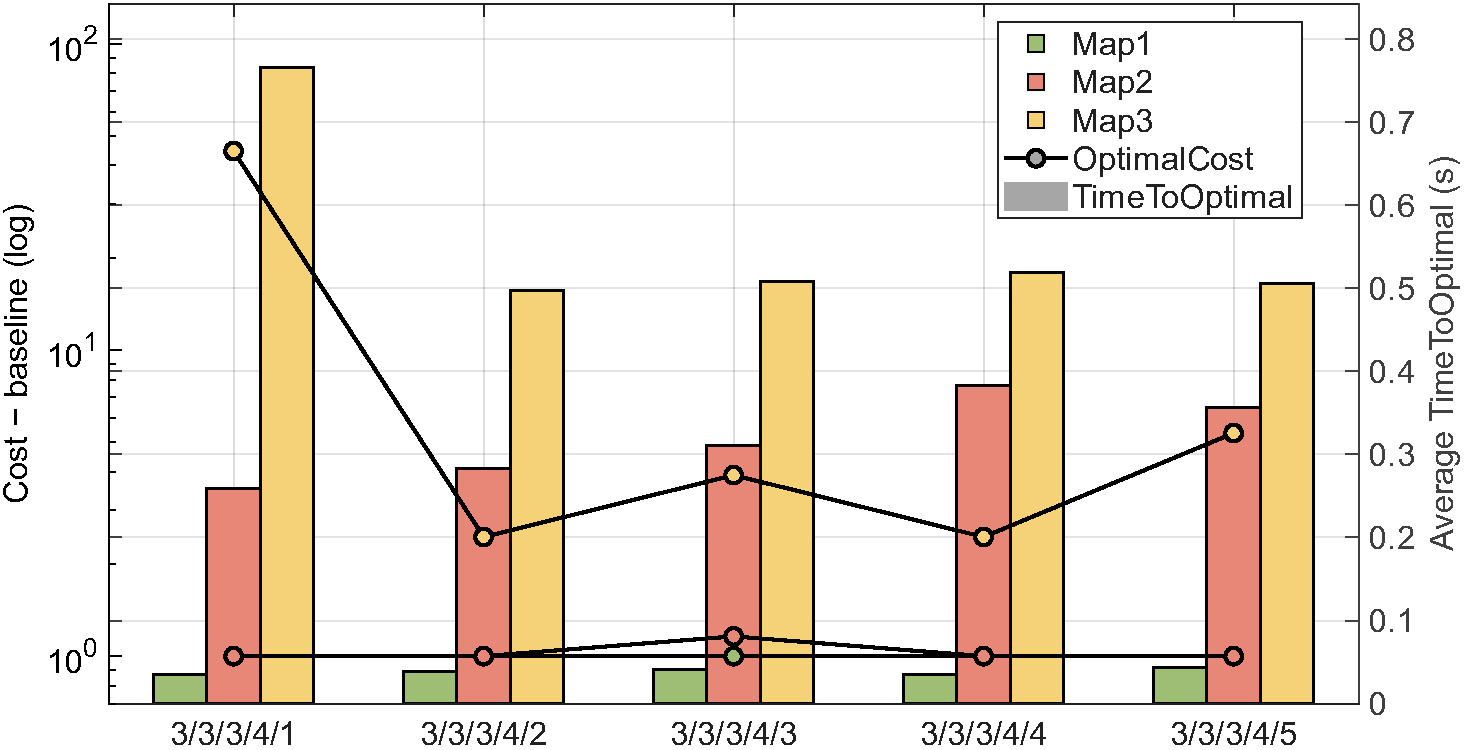
\includegraphics[width=0.32\textwidth]{figures/Sensitivity_Cost&Time_k}
\caption{Cost and computation time of each parameter level on Map~1, Map~2, and kroB100.}
\label{fig:sens_cost_time}
\end{figure*}

\begin{figure}[!ht]
\centering
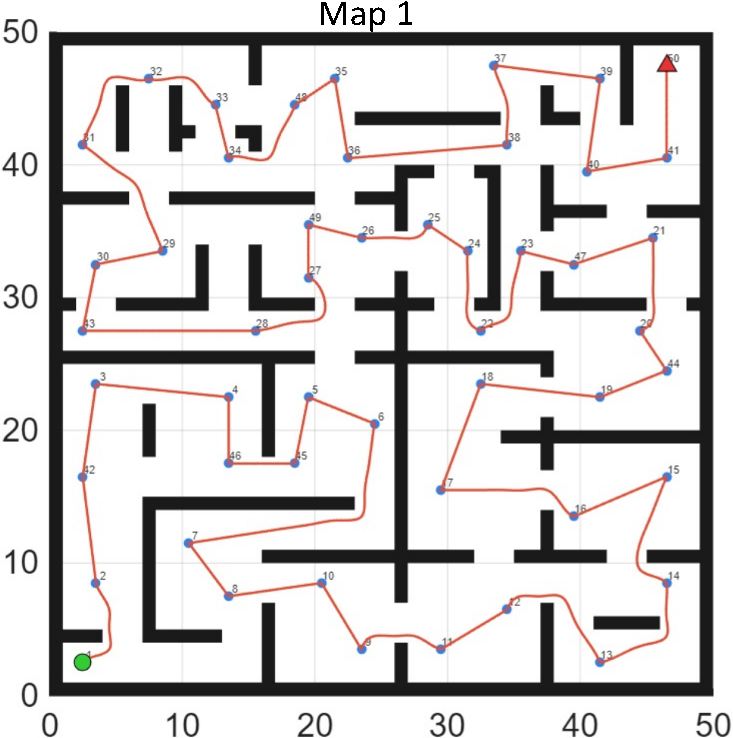
\includegraphics[width=1.55in]{figures/DifTSP_path_Map1_My}\hfil
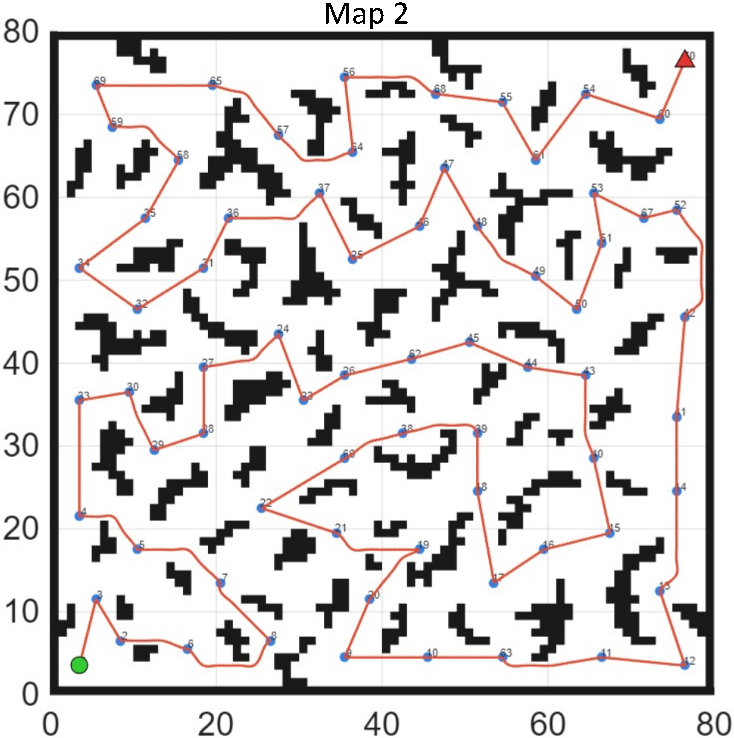
\includegraphics[width=1.55in]{figures/DifTSP_path_Map2_My}\\
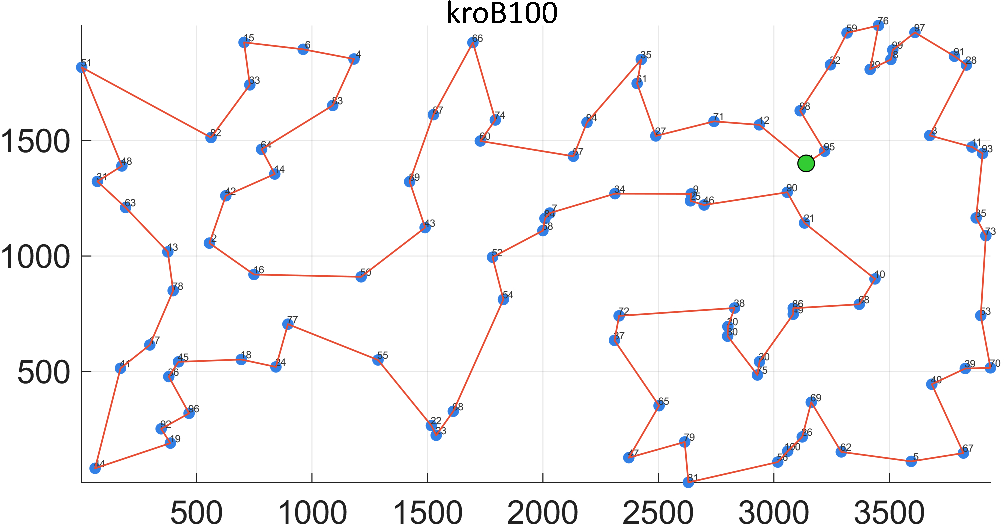
\includegraphics[width=2.5in]{figures/DifTSP_path_kroB100_My}
\caption{Paths planned by the algorithm on Map~1, Map~2, and kroB100 under the default parameter settings.}
\label{fig:sens_paths}
\end{figure}

This group of experiments examines the sensitivity of MMAS-VND-CL to five key hyperparameters, namely the number of ants $n_{\mathrm{ants}}$, the greedy selection probability $q_0$, the late-stage local-search ratio $y_{\max}$, the elite ratio $r_{\mathrm{elite}}$, and the candidate-list size $k$. Five parameter levels are first defined for each of these five parameters, as shown in Table~\textcolor{blue}{\ref{tab:levels}}. The level settings of subsequent experimental groups are denoted by the combined form $n_{\mathrm{ants}}/q_0/y_{\max}/r_{\mathrm{elite}}/k$. A single-factor design is adopted in the experiments: only one parameter is varied over its five levels at a time, while the remaining parameters are kept at their defaults. A total of 21 single-factor configurations are implemented, among which the experimental groups 3/3/3/4/2 correspond to the default parameter-level combination. Each group is run independently 40 times on Map~1, Map~2, and kroB100. Evaluation considers not only the best cost, but also the mean cost with standard deviation, the success rate, and the average convergence time. Complete numerical results for all configurations have been organized into the sensitivity results table in the accompanying experimental-data document and are not listed one by one in the main text. The cost--time trends are shown in Fig.~\textcolor{blue}{\ref{fig:sens_cost_time}}, and the path morphology under the default parameters is shown in Fig.~\textcolor{blue}{\ref{fig:sens_paths}}.

\begin{table}[!t]
\caption{Parameter Levels Used in the Sensitivity Analysis}
\label{tab:levels}
\centering
\setlength{\tabcolsep}{4pt}
\begin{tabular}{lccccc}
\toprule
\multirow{2}{*}{Parameter} & \multicolumn{5}{c}{Parameter Levels} \\
\cmidrule(lr){2-6}
 & Level 1 & Level 2 & Level 3 & Level 4 & Level 5 \\
\midrule
$n_{\mathrm{ants}}$ & 10 & 20 & \textbf{40} & 60 & 90 \\
$q_0$ & 0.10 & 0.30 & \textbf{0.45} & 0.60 & 0.90 \\
$y_{\max}$ & 0.10 & 0.20 & \textbf{0.40} & 0.60 & 0.90 \\
$r_{\mathrm{elite}}$ & 0.1 & 0.3 & 0.5 & \textbf{0.7} & 0.9 \\
$k$ & 3 & \textbf{9} & 15 & 30 & 60 \\
\bottomrule
\end{tabular}
\end{table}

For Map~1, Map~2, and kroB100, the reference best costs are 352.56, 623.78, and 22141, respectively. From the perspective of the reference best cost, the sensitivity results in the accompanying experimental-data document show that all configurations are able to reach the same reference value. This indicates that MMAS-VND-CL has a strong ability to ``find a high-quality solution'' within a reasonable parameter range; what truly separates the configurations is the success rate, the mean cost, and the computation time. Combining these observations with Fig.~\textcolor{blue}{\ref{fig:sens_cost_time}}, the main conclusions are as follows: $q_0$ and $y_{\max}$ are the most sensitive (degradation is especially pronounced when $q_0$ is large and $y_{\max}$ is small), $n_{\mathrm{ants}}$ and $r_{\mathrm{elite}}$ are intermediate, and $k$ is relatively flat within a moderate range but collapses when it is too small. The default combination ($3/3/3/4/2$) strikes a relatively balanced trade-off among quality, stability, and time, and is therefore fixed for subsequent experiments. The parameters are discussed individually below.

In terms of parameter regularity, $q_0$ and $y_{\max}$ are the most sensitive, $n_{\mathrm{ants}}$ and $r_{\mathrm{elite}}$ are intermediate, and $k$ is relatively flat within a moderate range but collapses when it is too small. The parameter $q_0$ controls the balance between exploitation and exploration in the pseudo-random transition. When it is set to 0.90 (nearly pure greedy), the ant colony almost always locks onto the currently highest-scoring candidate, and the pheromone rapidly collapses onto a small number of edges: the success rate on kroB100 drops to 57.5\% with the standard deviation rising to 45.78, and Map~2 reaches only 70\%. Lowering $q_0$ to 0.10--0.30 preserves a 100\% success rate, but the computation time becomes noticeably longer (about 490--720~ms). The parameter $y_{\max}$ determines the intensity of late-stage VND refinement. At $y_{\max}=0.10$, the lack of intensified late-stage local search leaves the success rate on Map~2 at only 62.5\%. At $y_{\max}=0.90$, the success rate instead declines, presumably because overly strong local search prematurely locks some runs into suboptimal structures.

Increasing $n_{\mathrm{ants}}$ from 10 to 40 raises the success rate on Map~2 from 92.5\% to 100\% and that on kroB100 from 95\% to 97.5\%. When the population is too small, pheromone updates are easily biased by a few individuals and the variance increases. Further increasing $n_{\mathrm{ants}}$ to 60--90 no longer improves the success rate, while the computation time increases by about 20\%--60\%; this is a ``sufficient and inexpensive'' compromise. When $r_{\mathrm{elite}}$ is set to 0.1--0.5, the success rate on kroB100 can reach 100\% or nearly 100\%, whereas over-elitization at 0.9 reduces it to 92.5\%. Over the range 9--60, $k$ has little effect on the cost, but at $k=3$ candidate pruning filters out promising edge exchanges as well, the success rate falls to 42.5\%, and the computation time rises to about 765.9~ms.

It should also be pointed out that no single configuration dominates on every metric; evaluation must trade off hit quality, stability, and computation time. The default combination $40/0.45/0.40/0.7/9$ achieves a 100\% hit rate with zero variance on Map~1 and Map~2, and on kroB100 attains a 97.5\% success rate with a relatively small standard deviation in about 500~ms. Its overall performance is the most balanced, and therefore the subsequent ablation and algorithm-comparison experiments all adopt this configuration.
